\documentclass[a4paper,twocolumn,12pt]{article}
\usepackage{url}
\usepackage{graphicx}

\title{Interrupt Controller Datasheet}

\author{Koen Martens\\
        \texttt{kmartens@sonologic.nl}}

\begin{document}
\maketitle

\section{Introduction}

The Sonologic Programmable Interrupt Controller is a WISHBONE B4 \cite{wishbone} compliant interrupt controller. The interrupt controller is a WISHBONE slave device. It offers a variable amount of interrupt banks. Each bank has three configuration registers and one status register. An interrupt bank contains a variable amount of interrupt lines. Interrupt lines can trigger on the rising edge, falling edge and level. Interrupt lines can be individually masked.

Figure \ref{fig:block_diagram} contains the block diagram of the programmable interrupt controller. 

\begin{figure}[h]
    \centering
    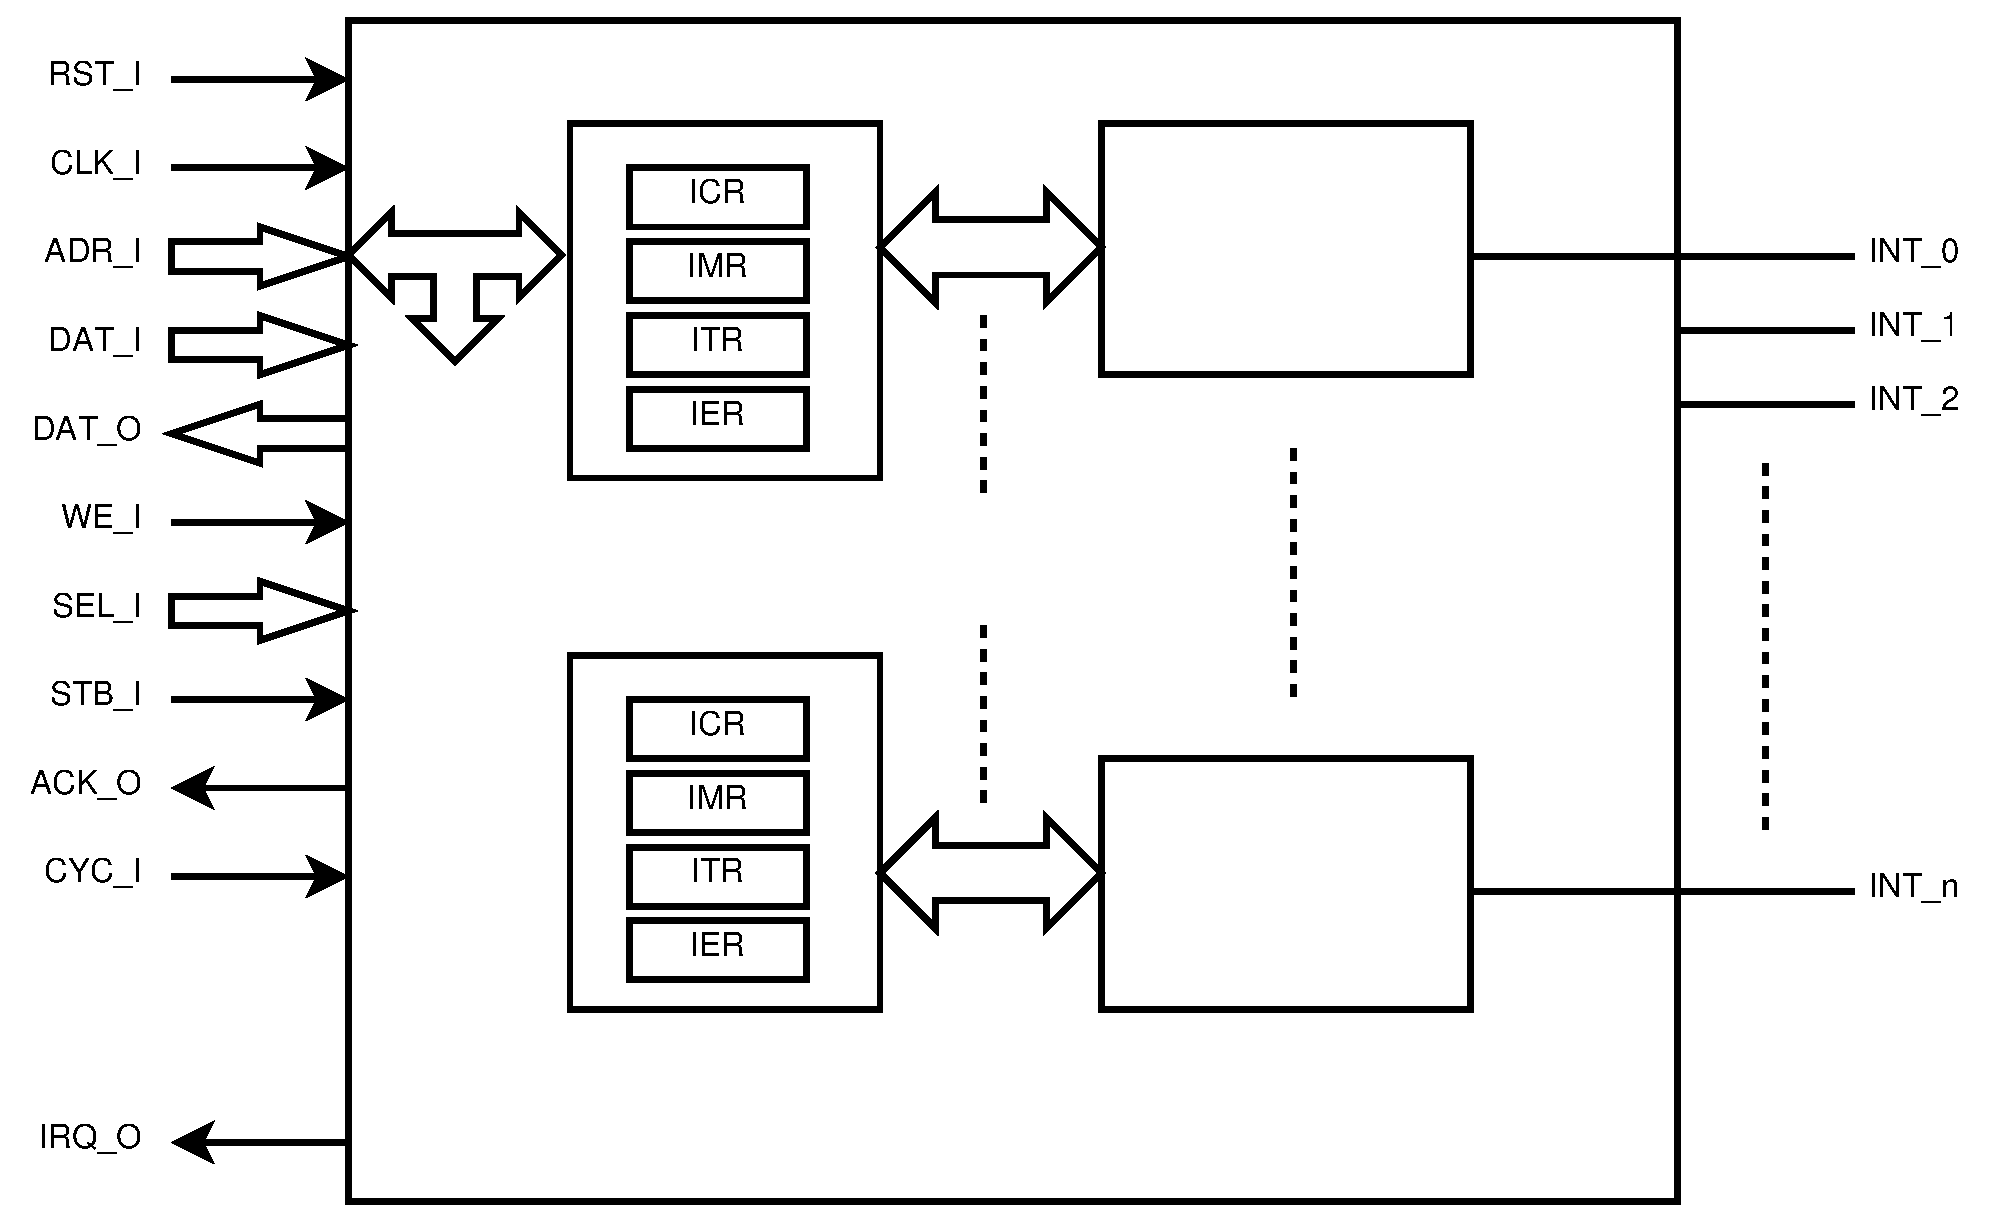
\includegraphics[width=7cm]{pic_block_diagram}
    \caption{Block diagram}
    \label{fig:block_diagram}
\end{figure}

\section{Notation}

\begin{description}
    \item[BUS(1:0)] Bit 1 downto 0 of bus BUS.
\end{description}

\section{Design unit}

\subsection{Design constraints}

The address bus (ADR\_I) must be able to address each register in each register bank. Each register bank occupies 4 words. The two least significant bits of the address bus address each of the 4 registers. The minimum length of the address bus is two bits when the design has only one register bank.

For additional register banks the bits down to the third least significant bit select the the register bank. To address N\_BANKS register banks the 

\section{Application}

The reference design uses the gmzpu \cite{gmzpu} cpu with the zwishbone controller. The reference application of the design entity has a data width of 32 bits and an address width of 16 bits. One interrupt bank (of 32 interrupt lines) is used.

\begin{thebibliography}{9}

\bibitem{wishbone} OpenCores \emph{Wishbone B4, WISHBONE System-on-Chip (SoC)Interconnection Architecture for Portable IP Cores} \url{http://opencores.org/opencores,wishbone} 2010.

\bibitem{gmzpu} Sonologic \emph{gmzpu github repository} \url{http://github.com/sonologic/gmzpu}.
\end{thebibliography}

\end{document}

